\documentclass[journal]{vgtc}                % final (journal style)
%\documentclass[review,journal]{vgtc}         % review (journal style)
%\documentclass[widereview]{vgtc}             % wide-spaced review
%\documentclass[preprint,journal]{vgtc}       % preprint (journal style)
%\documentclass[electronic,journal]{vgtc}     % electronic version, journal

%% Uncomment one of the lines above depending on where your paper is
%% in the conference process. ``review'' and ``widereview'' are for review
%% submission, ``preprint'' is for pre-publication, and the final version
%% doesn't use a specific qualifier. Further, ``electronic'' includes
%% hyperreferences for more convenient online viewing.

%% Please use one of the ``review'' options in combination with the
%% assigned online id (see below) ONLY if your paper uses a double blind
%% review process. Some conferences, like IEEE Vis and InfoVis, have NOT
%% in the past.

%% Please note that the use of figures other than the optional teaser is not permitted on the first page
%% of the journal version.  Figures should begin on the second page and be
%% in CMYK or Grey scale format, otherwise, colour shifting may occur
%% during the printing process.  Papers submitted with figures other than the optional teaser on the
%% first page will be refused.

%% These three lines bring in essential packages: ``mathptmx'' for Type 1
%% typefaces, ``graphicx'' for inclusion of EPS figures. and ``times''
%% for proper handling of the times font family.

\usepackage{mathptmx}
\usepackage{graphicx}
\usepackage{times}

%% We encourage the use of mathptmx for consistent usage of times font
%% throughout the proceedings. However, if you encounter conflicts
%% with other math-related packages, you may want to disable it.

%% This turns references into clickable hyperlinks.
\usepackage[bookmarks,backref=true,linkcolor=black]{hyperref} %,colorlinks
\hypersetup{
  pdfauthor = {},
  pdftitle = {},
  pdfsubject = {},
  pdfkeywords = {},
  colorlinks=true,
  linkcolor= black,
  citecolor= black,
  pageanchor=true,
  urlcolor = black,
  plainpages = false,
  linktocpage
}



\hyphenation{cellPack}

\usepackage{xcolor}
\definecolor{darkgreen}{RGB}{0,158,0}
\definecolor{green}{RGB}{145,209,145}
\definecolor{grey}{RGB}{220,220,220}

% ---------------------------------------------------------------------
% EG author guidelines plus sample file for EG publication using LaTeX2e input
% D.Fellner, v1.17, Sep 23, 2010


\title[Visibility Equalizer]%
      {\textcolor{darkgreen}{------}\textcolor{green}{-----}\textcolor{grey}{---} Visibility Equalizer \textcolor{grey}{---}\textcolor{green}{-----}\textcolor{darkgreen}{------} \\ Cutaway Visualization of Mesoscopic Biological Models}

% for anonymous conference submission please enter your SUBMISSION ID
% instead of the author's name (and leave the affiliation blank) !!
\author[Le Muzic, Mindek et al.]
       {M. Le Muzic\thanks{Both first authors contributed equally. ~~~~~~~~~~~~~~~~~~~~~~~~~~~~~~~~~~~~~~~~~~~~~~~~~~~~~~~ Contact: \{mathieu | mindek\}@cg.tuwien.ac.at}$^{1}$,
        P. Mindek$^{1}$,
        J. Sorger$^{1,2}$,
        L. Autin$^{3}$,
        D. Goodsell$^{3}$,
        and I. Viola$^{1}$        
        \\
%For Computer Graphics Forum: Please use the abbreviation of your first name.
         $^1$TU Wien, Austria \hspace{4mm}$^2$VRVis Research Center, Vienna, Austria \hspace{4mm}$^3$The Scripps Research Institute, La Jolla, California, USA
       }

%\author[275]{Submission ID 275}

% ------------------------------------------------------------------------

% if the Editors-in-Chief have given you the data, you may uncomment
% the following five lines and insert it here
%
% \volume{27}   % the volume in which the issue will be published;
% \issue{1}     % the issue number of the publication
% \pStartPage{1}      % set starting page


%-------------------------------------------------------------------------
\begin{document}

\teaser{
% 
\includegraphics[width=\linewidth]{eg_new}
% \centering
%  \caption{New EG Logo}
%\label{fig:teaser}

\centering
\subfloat[]{\label{fig:res:w0}\includegraphics[width=0.25\linewidth]{figures/res-w0.eps}}
\subfloat[]{\label{fig:res:w3}\includegraphics[width=0.25\linewidth]{figures/res-w8.eps}}
\subfloat[]{\label{fig:res:w1}\includegraphics[width=0.25\linewidth]{figures/res-w4.eps}}
\subfloat[]{\label{fig:res:w2}\includegraphics[width=0.25\linewidth]{figures/res-w6.eps}}

\caption{\label{fig:teaser}The workflow of our method for a model of HIV surrounded with blood plasma proteins. (a) Entire dataset is shown. The blood serum (shown in red) is occluding the virus. (b) Clipping objects are added to selectively clip molecules to reveal the HIV capsid. (c) The illustrator decides to show more of the matrix protein (shown in blue), so their clipping is disabled. However, they are now occluding the view of the capsid. (d) The probabilistic clipping has been used to selectively remove those matrix proteins occluding the capsid, but some of them are left in the scene to indicate the presence of this type of protein on the virus membrane. The capsid has been clipped with view-space clipping to reveal its internals.}
%\subfloat[]{\label{fig:res:w0}\includegraphics[width=0.25\linewidth]{figures/res-w0.eps}}
%\subfloat[]{\label{fig:res:w1}\includegraphics[width=0.25\linewidth]{figures/res-w1.eps}}
%\subfloat[]{\label{fig:res:w2}\includegraphics[width=0.25\linewidth]{figures/res-w2.eps}}
%\subfloat[]{\label{fig:res:w3}\includegraphics[width=0.25\linewidth]{figures/res-w3.eps}}

%\subfloat[]{\label{fig:res:w4}\includegraphics[width=0.25\linewidth]{figures/res-w4.eps}}
%\subfloat[]{\label{fig:res:w5}\includegraphics[width=0.25\linewidth]{figures/res-w5.eps}}
%\subfloat[]{\label{fig:res:w6}\includegraphics[width=0.25\linewidth]{figures/res-w6.eps}}
%\subfloat[]{\label{fig:res:w7}\includegraphics[width=0.25\linewidth]{figures/res-w7.eps}}
\vspace{10mm}
}

\maketitle

\begin{abstract}
In scientific illustrations and visualization, cutaway views are often employed as an effective technique for occlusion management in densely packed scenes.
We propose a novel method for authoring cutaway illustrations of mesoscopic biological models.
In contrast to the existing cutaway algorithms, we take advantage of the specific nature of the biological models. 
These models consist of thousands of instances with a comparably smaller number of different types.
Our method constitutes a two stage process.
In the first step, clipping objects are placed in the scene, creating a cutaway visualization of the model.
During this process, a hierarchical list of stacked bars inform the user about the instance visibility distribution of each individual molecular type in the scene.
In the second step, the visibility of each molecular type is fine-tuned through these bars, which at this point act as interactive visibility equalizers. 
%The visibility equalizers give illustrators precise control over how much percent of each type of molecule should be visible in front of the cutting object. 
%Thus enabling them to quickly and efficiently create visualizations of biological models that provide insights  which would have taken them to manually recreate.
An evaluation of our technique with domain experts confirmed that our equalizer-based approach for visibility specification was valuable and effective for both, scientific and educational purposes.




%In molecular biology and similar fields, knowledge transfer is commonly carried out through schematic illustrations.
%Traditionally, illustrations of biological processes on the molecular level have been created by manual hand drawing.
%Nowadays, complex models of various biochemical structures and micro-organisms exist.
%These models can be utilized in creating computer-generated biological illustrations through various molecular-visualization algorithms.
%When using such algorithms, it is beneficial for illustrators to be able to apply techniques common in traditional illustration, such as cutaway views.
%In this paper, we propose a method for enhancing real-time molecular-visualization algorithms with the capability to apply cutaway views.
%In contrast with existing cutaway algorithms, we take advantage of the specific nature of the biochemical models, which consists of multiple instances of a limited number of different molecular types.
%Our approach to cutaway views allows the illustrators to reintroduce some of the removed instances into the scene to communicate the presence of the given molecular type, yet maintaining the visibility of the internal structures of the model.
%This process is enabled through a novel interaction method for controlling the visibility in the instance-based scene. We refer to this method as visibility equaliser.


%In this paper, we propose a method for enhancing real-time molecular-visualization algorithms with the capability to display cutaway views.
%Such an option is beneficial to biological illustrators, since the technique of cutaway display is ubiquitously applied in traditional illustration.
%In contrast with existing algorithms for creating cutaway views, we take advantage of the specific nature of the biochemical models, which consist of multiple instances of the limited number of different molecular types.
%We are able to create comprehensible illustrations of complex models by reintroducing some of these instances in the cutaway parts of the rendered illustration.
%The main contribution of this paper is an interaction mechanism which allows the illustrators to precisely control the amount of instances of different molecular types in the illustration, while maintaining the desired information value.

\begin{classification} % according to http://www.acm.org/class/1998/
\CCScat{Computer Graphics}{I.3.3}{Picture/Image Generation}{Viewing algorithms}
\end{classification}

\end{abstract}

\clearpage


\section{Introduction}\label{sec:intro}

Molecular biology is an emerging field that is characterized by rapid advances of the current state of knowledge.
New discoveries have to be communicated frequently to a large variety of audiences.
However, due to their structural and phenomenal complexity, it is challenging to convey the discoveries of molecular phenomena. On a mesoscale level, where thousands or millions of macromolecules form a given structure, this challenge is amplified by the presence of multiple spatio-temporal scales. Currently, illustrations are the most widely-used form of communicating mesoscale structures. To reveal the internal composition of mesoscale structures such as viruses or bacteria, illustrators often employ clipping, section views or cutaways in their work.

%The traditional pipeline for creating scientific illustrations of molecular structures starts with gathering the required knowledge for building models that convey the newly discovered insights.
%Illustrators then create sketches, in which the relevant internal and external regions of these structures are uncovered.
%To achieve this, occlusion management techniques, such as \emph{cutaways} are applied.
%Cutaways remove specific outer parts of the organism model, so that internal structures become visible. 
%When biologists come up with new findings that are not depicted in the existing illustration, the conceptual layout of the original illustration might not be valid anymore.
%The whole illustration process has to be repeated, in the worst case from the beginning, which is cumbersome and time consuming.
%Such a cycle can take months or even years to complete.


Considering the rapid evolution of knowledge in the field of biology, it is necessary to adapt the traditional illustration pipeline so that new knowledge can be easily added into illustrations, instead of tediously redrawing the entire structure.
Virtual 3D models of cells and other mesoscale molecular structures can be utilized for these purposes.
Biologists have designed tools, such as \emph{cellPACK} \cite{cellpack}, to procedurally generate 3D models that represent the structure of micro-organisms such as viruses, or entire cells at atomic resolution.
Based on a set of input parameters, individual molecules are algorithmically assembled into these complex organic static structures. 
The parameter set consists of a specification of molecular types, concentrations and spatial distribution that define where are the instances distributed in a given compartment. 
The resulting 3D models, in the most complex cases, may consist of thousands of various molecular types, which in turn, may result in millions of molecules and billions of atoms.
The instances are densely packed within the predefined compartments, to replicate the actual molecular crowding phenomena prevailing in living organisms.
Due to the high density of these scenes, inner structures that are essential for conveying the functioning of the organism remain hidden.
It is therefore important to develop visualization techniques that would procedurally reproduce the occlusion management methods used in traditional illustration.
Currently, this is achieved by placing clipping objects in the scene, which remove specified parts of the displayed model. 
However, illustrators have to make sure that the essential information, e.g., the ratio of multiple molecular ingredients, is represented and not either hidden in the volume or clipped away (Fig. \ref{fig:hiv0}). 
To do this, they would need to visually inspect the presence of each single ingredient in the resulting visualization (Fig. \ref{fig:hiv1}).
%However, in order to know how many instances have already been removed, and which molecular types are still sufficiently represented in the scene, the illustrator has to continuously check and compare the modeled scene against the gathered data and tediously confirm whether the essential information is still represented.
%As a tangible example, let us assume we have to confirm the presented ratio of multiple molecular ingredients (Fig. \ref{fig:which}a) in an illustration. 
%By clipping through the center of a 3D model, many structures can be revealed (Fig. \ref{fig:which}b). 
%However, for dozens of molecular types, it would be tedious to manually check whether all are displayed, or if some have been completely removed or not yet revealed through the clipping.
%However, to find out which of these ingredients have been actually shown by the clipping and which are completely cut or not yet revealed, one would need to manually check the presence of each single ingredient in the resulting visualization.

To alleviate this process, we present our first contribution: a method that quantifies the overall visibility of the model contents. We display a stacked bar for each molecular type that encodes the ratio of visible, clipped, and occluded instances of the respective type for the current viewpoint and clipping setting. 
During the process of placing clipping objects in the scene, these bars continuously reveal molecular types that are underrepresented or overrepresented. 
This enables the illustrator to modify the placement of the clipping objects in such a way that every molecular type is adequately represented in the scene. We call this the coarse level of the visibility specification process.

To preserve important structures that would be removed by clipping objects such as cutting planes, traditional illustrations also often reintroduce parts of them in front of the revealed cross sections. 
In Figure \ref{fig:hiv1}, for instance, the glycoproteins (yellow molecules) of the HIV particle that are not occluding the object of interest, in this case the capsid containing the RNA, are left in the illustration to communicate their presence on the surface of the virus (Fig. \ref{fig:hiv0}).
In this way, the main components of the virus particle can be illustrated in a single image.
%Simple cutaway however, only achieve cross sections.
%In traditional illustration, fine-level visibility specification is often utilized as well.
%To communicate the biology knowledge well, the illustrations have to sometimes display molecular instances which would be impossible to specify with the simple clipping objects, such as cutting planes.%An example is shown in Figure \ref{fig:hiv}.
%Figure \ref{fig:hiv0} shows an illustration of an HIV particle.
%In Figure \ref{fig:hiv1}, a cutting plane is used to reveal internal structures of the virus - the capsid containing the RNA.
%Some of the glycoproteins (yellow molecules) are left in the illustration to communicate their presence on the surface of the virus particle.
%In particular, those glycoproteins which are not occluding the object of interest, were chosen to be kept in the illustration providing the contextual information.
The process of fine-tuning the visibility is extremely time-consuming, as the illustrator has to manually pick individual molecular instances to be reintroduced or removed from the scene. %in order to preserve important information whily not occlude occluding 
%This might be done to control the under and over representation of some of the molecular types, removing instances occluding important aspects of the model, suggesting shapes, etc.

\begin{figure}[t]
\centering
\subfloat[]{\label{fig:hiv0}\includegraphics[width=0.495\linewidth]{figures/which0.eps}}
\subfloat[]{\label{fig:hiv1}\includegraphics[width=0.495\linewidth]{figures/which1.eps}}
\caption{\label{fig:which} (a) Various types of protein molecules and (b) their embedding into a mesoscale  model. It is a demanding task to determine which molecular types are visible and how many of their instances are shown.}
\vspace{-5mm}
\end{figure}


To speed up this visibility fine-tuning process, we propose our second contribution: a novel method for managing the visibility of instances. Instead of binary enabling or disabling the presence of all instances for a given molecular type, we offer the possibility to show a desired number of them.
The main purpose of this approach is to increase the visibility of hidden structures by removing redundant parts of occluding instances while preserving some of them.
An analogy of this approach can be drawn with ``Screen-Door Transparency'', a trivial way to obtain transparency in computer graphics by placing small holes in a polygon to reveal what is present behind.
Additionally, we propose the novel metaphor of the \emph{visibility equalizer} for controlling efficiently this effect.
%To significantly speed up this visibility fine-tuning process, we propose the novel metaphor of the \emph{visibility equalizer} as our main technical contribution.
To explain its role, we use the metaphor of hi-fi sound reproduction where the \textit{volume control} is used for adjusting the output sound \textit{uniformly} on all frequencies. 
Such a mechanism corresponds to our coarse-level visibility specification of the clipping objects, where all molecular types are uniformly removed from the clipped regions.
However, hi-fi sound systems also allow users to fine-tune the volume levels of individual frequency bands through an \emph{equalizer}.
Following this metaphor, the visibility levels of molecular types are represented as stacked bars that form our visibility equalizer.
All visibility bars are interactive, thus allowing the user to adjust desired levels just as with a sound equalizer. After drawing relation to previously proposed visibility management techniques in the next section, we will discuss the technique of visibility equalizers in further detail in the remaining sections of the paper.
%Individual intervals on each bar can be dragged to increase or decrease the visibility of the individual molecular types within the scene, given the specified clipping objects. 
%This interactive element effectively turns the stacked bars into visibility equalizers for the molecular models - and as such presents the main technical contribution of this paper.
%When interacting with the visibility equalizer, the artist or biologist can intuitively achieve expressive cutaway designs in a fraction of the time that would be needed for manual visibility adjustments.
%The conceptual contribution of this work is demonstration of a scenario where a visualization metaphor, such as the stacked bar chart in our case, can serve as a user interface for performing a specific task, in our case authoring a cutaway design. We expect to see further cases where (information) visualization is simultaneously the user interface.

%\noindent{Our main contributions are:} %\begin{itemize}  \item a new workflow for illustrator-authored cutaway illustrations from mesoscale 3D structural models  \item a new visual metaphor of visibility equalizers with which allows users to fine tune the cut-away design so that visibility is distributed among the molecular types as desired by the illustrator.\end{itemize}

\begin{comment}

To speed-up the fine tuning process we propose a novel method for clipping instances using a fuzzy approach. 
In addition to either entirely show or remove instances of a given ingredient by the clipping object, we offer the possibility to show only an arbitrary number of these instances.
The main advantage of this approach is that we are able to increase the visibility of hidden structures while preserving potentially important, but redundant occluding molecules.
An analogy of this approach can be drawn here with ``Screen-Door Transparency'', which is a trivial way to obtain transparency in computer graphics, by simply placing holes in the polygon to reveal what is present behind.

\end{comment}



\begin{comment}

In the field of molecular biology, micro-biology, and medicine, illustrations are essential for the inter- and intra-disciplinary knowledge transfer.
Over the years, illustrators have developed various techniques for capturing specific aspects of the displayed objects and processes.
One of the most common methods utilized in the technical illustration are so-called \emph{cutaway views}.
When a cutaway view is applied, parts of the illustrated object are left out, such as if they were physically cut away.
In this way, internal structures, which are to be communicated by the illustration, can be shown.

Creating hand-drawn illustrations of complex polymolecular structures, or even entire microorganisms, is an extremely tedious task. Such structures can contain hundreds of thousands of molecules.
Therefore, to communicate the intended message, it is often necessary to adequately simplify the structure in question.
The illustration then consists of appropriate abstractions, while certain amount of information is lost.

A different approach is to utilize computational models of the structures which are to be illustrated, and utilizing software packages for visualization of these models.
Such models, typically generated through simulation and statistical modelling, consists of large numbers of instances of several molecular types.
The different molecular types contained within the model represent the chemical composition of the modelled object, while the distributions of the instances of the individual types represent the concentrations of the respective chemical compounds.
High number of molecular instances, as well as their large densities, often make task of visualizing such models non-trivial.
The advantage of this approach is the possibility to generate illustrations exhibiting high degree of accuracy, which would require extremely high effort.

When utilizing the molecular models for the illustrative purposes, algorithmic equivalents of the traditional illustrative techniques are often employed.
For instance, software packages for computer-aided illustration often offer an option to manipulate and apply culling objects for creating cutaway views of the illustrated models or scenes.
The culling objects work in such a way that the part of the rendered scene enclosed by the surface of the cutting object is removed, thus making previously occluded structures visible.

%Cutaways views are essential in illustration of processes on the microscopic scale. These processes are often demonstrated on polymolecular models, where large number of molecular instances form complex nested structures. Such structures would be impossible to visualize when the model is displayed as a whole, thus creating a need for the cutaway views.

Simple culling objects are not always sufficient for the illustrative purposes. Sometimes, it is necessary to reintroduce parts of the scene that has been culled away in order to increase the informative value of the illustration. An example is shown in Figure \ref{fig:hiv}.
Figure \ref{fig:hiv0} shows an illustration of an HIV particle.
In Figure \ref{fig:hiv1}, a cutaway view is used to reveal internal structures of the virus - the capsid containing the RNA.
Some of the glycoproteins (yellow molecules) are left in the illustration to communicate their presence on the surface of the virus particle.
In particular, those glycoproteins which are not occluding the object of interest, were chosen to be kept in the illustration providing the contextual information. In this way, the main components of the virus particle can be illustrated in a single image.

In general, illustrators choose such placements of the culling objects that only unimportant parts of the scene are removed and no essential information is lost.
Specifically in molecular visualization, it is often desired that the culling objects are positioned so that all molecular types are represented in the generated scene.
However, the placement of the culling objects also needs to correspond with the geometrical structure of the model, so that it is obvious what are the artificial cuts introduced in the illustration, and what is their purpose.
Given the high complexity inherent to most of the molecular models, meeting both of these requirements at the same time is a difficult task.
With each additional culling object that the illustrator introduces into the scene, it gets progressively more difficult to keep overview of which molecular types are still represented in the scene in sufficient amounts.

To alleviate this problem, we propose \emph{Visibility Equalizer}.
It is a visualization element which displays a histograms of the individual molecule types present in the scene.
These histograms show the total numbers of molecules of each type in the model, numbers of molecules cut away by the clipping objects, and numbers of molecules of each type which are actually visible from the current viewpoint.
By showing these histograms, the illustrator is informed about the information value of the illustration at any given time during the creative process.

We focus on real-time visualization tools that can be used for illustration of molecular data.
In these scenarios, the user does not have direct control over the presented content, in contrast to a scenario where the content is created by manually placing individual molecules into the scene.
Therefore, Visibility Equalizer provides essential information about the scene while multiple culling objects are placed and dynamically manipulated.

\end{comment}




\section{Related Work}
Related work can be categorized into occlusion management techniques and molecular visualization. We will concentrate on the former, according to the focus of this paper.

\subsection{Occlusion Management}
Related occlusion management techniques can be categorized into object centric approaches and transfer function based approaches. In object centric approaches, the geometry or parts of the volume that are obstructing one or more particular objects of interest are (partially) removed. In transfer function based approaches, the user assigns importances to intervals of the volume data values.

\noindent
\textbf{Object Centered Approaches.}
Cutaway and ghosting techniques were first introduced by Feiner \& Seligmann \cite{feiner92} in 1992.
 %as an automated approach for generating illustrations that consider the occlusion of user defined objects. In 2002, Diepstraten et al. \cite{diep02} picked up the technique again and defined a set of rules for computer-based rendering of technical illustrations to achieve a view-dependent transparency model that mimics the ghosting techniques of technical illustrations. They later extended these rules for interactive cutaway illustrations \cite{diep03}.
%Analogous to the cutaways for polygonal representations, Weiskopf et al. \cite{weiskopf03} developed an interactive clipping technique for volume rendering that supports complex clipping geometries. In 2004, Viola et al. \cite{viola2004importance} developed an automated approach for focus \& context visualization for segmented volumetric objects. An assigned object importance determines the visibility priority for the segmented parts of the volume. Contextual information is kept in regions where the context does not occlude the feature of interest. Follow-up work focused on the definition of levels of sparseness and importance compositing for cutaway and ghosting calculations \cite{Viola05}. 
%In 2005, Viola \& Gr{\"o}ller \cite{violasmart05} give an overview of  "smart visibility" techniques. The term describes expressive visualization techniques that smartly uncover the most important features of the displayed data, such as cut-away views, ghosted views, and exploded views. 
Their work inspired several follow-up approaches \cite{diep02, diep03, weiskopf03, viola2004importance, Viola05, Kruger05} that were later summarized in the survey by Viola \& Gr{\"o}ller \cite{violasmart05} under the collective term of \textit{smart visibility} techniques. They coined this term to describe expressive visualization techniques that smartly uncover the most important features of the displayed data, i.e., cutaway views, ghosted views, and exploded views. 
%A. Kr{\"u}ger et al. \cite{Kruger05} combined visualization and interaction techniques such as cutaway views, silhouettes and color-coded distances  to improve the spatial perception of feature arrangement for surgical planning.  lymph nodes are emphasized using ghosted views to easily convey their spatial position.

Kr{\"u}ger et al. \cite{kruger06} developed a system that applies transparency and shading to enable focus\&context visualization in volume data sets with a simple point\&click interface.
%Li et al. \cite{Li07} developed an approach that allows interactive exploration of complex models, e.g., mechanical or anatomical, that requires the user to rig each part of the respective model. Based on the rigging, the system produces cuts that adhere to a set of rules that were inspired by anatomic and mechanical illustrations. 
Li et al. \cite{Li07} propose a cutaway design based on the geometry of the occluder in contrast to previous approaches that were based on the occludee.
Burns \& Finkelstein \cite{Burns08} applied the concept of importance-driven cutaways for volume data to polygonal models.
%The approach by Burns \& Finkelstein \cite{Burns08} for view dependent cutaways inspired our aperture that is discussed in section XXX. The cutaway shape is determined by the enlarged shape of the focus objects in the depth image. To preserve the information of the cut geometry, they apply shading and contouring/outlining of the cut surfaces, as well as ghosting of the cut geometry contours. 
Lawonn et al. \cite{lawonn16} extend this approach to present a composite technique that combines the visualization of blood flow with the surrounding vessel structures. %The structures visually encode the wall thickness as colored regions in order to preserve important context information. 
Baer et al. \cite{baer11} published a perceptual evaluation of smart visibility techniques for two ghosted view approaches in comparison to semi-transparent approaches. The results clearly favored the ghosted view techniques.
Sigg et al. \cite{sigg12} propose an approach for automatic cutaway box placement with optimized visibility for target features that are specified as degree-of-interest functions during interactive visual analysis of the volume data. Lidal et al. \cite{Lidal12} defined five design principles for cutaway visualization of geological models. %. They promote boxes as ideal cutaway shapes for emphasizing the shape and depth of focus features in layered structures, such as geological sediments. Illumination should effectively communicate the shape and spatial ordering inside the cutaway, as well as enhancing relationships between the focus features and the context. They define five design principles
%that we discuss in Section \textbf{XXX} in relation to our approach.
%A view dependent peel-away approach for volume data was proposed by Birkeland and Viola \cite{birkeland09}. 
The approach by Diaz et al. \cite{diaz12} preserves the relevant context information in volume clipping by allowing the user to extrude segmented surfaces such as bone structures from the clipping plane.

Since these approaches are object centered, they deal with (partial) occlusion of individual objects. For our data, partial or even complete occlusion of individual molecules is not an issue. The data is not composed of large singular entities such as polygonal or segmented volumetric objects where each single one has a semantic meaning. Instead, there are thousands or hundreds of thousands of instances that stem from only a couple of dozen molecule types. Therefore it does not matter if individual instances are occluded, as long as the structures that they form are preserved.
Our approach is therefore fundamentally different from existing occlusion management approaches as it combines principles from object centered and transfer function based approaches.


\begin{figure*}[t]
	\centering
	\includegraphics[width=\linewidth]{figures/__overview.eps}
	\caption{\label{fig:o}
		An illustration of the workflow with the visibility equalizer. 		
		Clipping objects filter-out elements in the data based on their type and location (1).
		The clipping is applied in serial, i.e., the output of a clipping object constitute de the input of the next one.
		The visibility information of the entire scene is routinely collected and updated in the visibility equalizer to keep the viewer informed about the current state of the data (2).
		The clipping parameters of a given clipping object can later on be refined by interacting with the bar charts of the visibility equalizer to offer more control on the clipping, such as fuzziness (3).		
		%Upon interaction with the bar charts, the properties of the selected clipping object is overridden to offer more control on the clipping, such as fuzziness.
		%The data can be displayed either without any clipping (\emph{S1}), with deterministic clipping defined by the clipping objects (\emph{S2}), or probabilistic clipping specified through the visibility equalizer (\emph{S3}). 
		%Lower part (technical overview): each clipping object filters the output of the previous one. 
		%The rendered image is used to update the visibility equalizer.
		%Interaction with the bars updates the scene to match the specification in the visibility equalizer.
		%(b) The technologies used in the workflow. 
		%The user can either use clipping objects to clip the data, or he can manipulate the visibility equalizers to modify clipping parameters of the clipping objects.
	}
\end{figure*}



\noindent
\textbf{Transfer Function Based Approaches.}
Since our molecule data is composed of a dense point cloud that resembles volumetric data on a non regular grid, our approach is also related to transfer function based approaches.
However, instead of a wide range of attribute values distributed over voxels, our data features a comparably smaller number of molecule types. This characteristic enables our visibility equalizer approach. %Our approach could also be applied to volumetric data by binning continuous attribute ranges into discrete ones.
The context-preserving volume rendering model \cite{Bruckner05} uses a function of shading intensity, gradient magnitude, distance to the eye point, and previously accumulated opacity to selectively reduce the opacity in less important data regions. Contours of surfaces that would be removed due to opacity, remain visible as the amount of illumination received is taken as a measure whether a point should be visible or not.
Burns et al. \cite{Burns07} propose a multimodal approach that combines CT scan data and real-time ultrasound data. Importance driven shading is used to emphasize features of higher importance that have been revealed through the ghosting.

In his PhD thesis \cite{phd-viola}, Viola presents an optimization strategy for automatically assigning visual mapping to voxels so that segmented objects in the volume are visible as specified by the user. Correa et al. \cite{correa11} used a similar approach for applying visibility directly to voxels, without the notion of segmented objects.
In our approach, we control visibility by interacting with the stacked bars of the visibility equalizer to modify the clipping object properties for each icndividual molecule type.
%In contrast to this work, the motivation for our proposed method is to design an interface for authoring cutaway illustrations of mesoscopic multi-molecular data. The properties of such data imply that each bin of our visibility equalizer, representing individual molecular ingredients, can be interacted with to change the properties of the clipping objects applied to the 3D scene.
%The notion of visibility histograms proposed by Correa et al. \cite{correa11} inspired our visibility equalizer metaphor. These histograms represent the distribution of visibility in a volume-rendered image and should help users manage a set of transfer function parameters to maximize the visibility of interesting intervals in the volume.
%Correa et al. \cite{correa11} present visibility histograms for specification of transfer functions for volume rendering. 
Ruiz et al. \cite{ruiz11} propose an approach for automatic transfer function op
timization by minimizing the informational divergence between a user specified target distribution and the visibility distribution captured from certain viewpoints. 

Transfer function based approaches are well suited for volumetric data that contains segmentable structures, such as the organs or bones in a medical scan. For molecular data this only holds partially true, as some types of molecules do indeed form continuous structures that could be made visible with a transfer function (e.g., membranes, nucleus). On the other side, within these structures there is a more noise-like distribution of these molecules that cannot be segmented into solid structures.



\subsection{Mutli-Scale Visualization of Molecular Structures}
%The visualization of the molecular structures in our approach is based on the publicly available cellView \cite{muzic15}. The tool is capable of rendering structures that are comprised of several billions atoms at interactive frame rates in multiple levels of detail.  
Lindow et al. \cite{lindow15} were the first to introduce a fast method for the real-time rendering of large-scale atomic data on consumer level hardware. They utilize instancing on the GPU to repeat these structures in the scene. For each molecule type, a 3D grid of the atoms is created and stored on the GPU. Falk et al. \cite{falk13} further refined the method with improved depth culling and hierarchical ray casting to achieve faster rendering performance for even larger scenes. 

A novel and more efficient approach for rendering large molecular datasets was later on introduced by Le Muzic et al. \cite{le2014illustrative}, which is based on brute-force rasterization rather than ray-tracing. 
To reduce the number of drawn geometries they rely on the tessellation shader to perform dynamic level-of-detail. 
Their approach allows switching between different degree of coarseness for the molecular structures on-the-fly, thus allowing the entire scene to be rendered in a single draw call efficiently, approaching zero driver overhead. 
As a follow up, they developed and released cellVIEW \cite{muzic15}, a tool designed for rendering large-scale molecular scenes, which was implemented with Unity3D, a popular 3D engine.
cellVIEW was primarily developed to showcase large molecular structures generated with cellPACK \cite{cellpack}, a tool developed to procedurally generate accurate and multi-scale models of entire viruses and cells.

Our visibility equalizer technique is built-upon cellVIEW, and is an attempt to improve the navigation and exploration of large molecular scenes generated with cellPACK.
cellVIEW leverages GPU computing and parallel programming to enable real-time rendering and therefore, to provide a smooth and responsive user-experience, the visibility equalizer was developed with the same programming paradigm.

%Other related work is concerned with illustrative molecular visualization. Grottel et al. \cite{grottel12} and Eichelbaum et al. \cite{eichelbaum13} propose ambient occlusion approaches for large molecular scenes in order to improve the depth perception in these complex structures. Parulek et al. \cite{parulek14} propose a continuous level of detail scheme for molecular data that offers gradual shape simplification for distant molecules based on a clustering of the atomic spheres.

%In the domain of dedicated mesoscopic molecular visualization, our approach is the first to introduce illustrative occlusion management techniques.




\input{pipeline.inc}

\input{poc.inc}
\section{Results and Performance Analysis}

To showcase the capabilities of our method, we applied it to three different mesoscale molecular scenes. 
For the rendering, we used cellVIEW \cite{muzic15}, a tool designed to efficiently render large molecular scenes on the GPU and implemented with Unity3D. 
The different datasets have been generated by the domain experts with cellPACK \cite{cellpack}, a modeling tool for procedural generation of large biomolecular structures.
cellPACK summarizes and incorporates the most recent knowledge obtained from structural biology and system biology to generate comprehensive mesoscale models. 
Based on experimentally obtained data (such as proteins structure, concentration and spatial distribution), the tool is able to generate entire models of viruses and cells via a packing method based on collision constraints.

%The results of the packing with cellPACK is stored in a file and loaded in cellVIEW afterwards.  
%The file generated by cellPACK contains the description of the scene, namely, position, rotation and type of each individual instances.
%In order the load and display the scene, cellVIEW reads the instances information from the file and uploads it on the GPU memory thus allowing fast read accesses from the rendering pipeline.

\begin{figure*}[t]
\centering
\subfloat[]{\label{fig:res:gh3}\includegraphics[width=0.33\linewidth]{figures/res-gh3.eps}}
\subfloat[]{\label{fig:res:myco}\includegraphics[width=0.26\linewidth]{figures/mycoplasma.eps}}
\subfloat[]{\label{fig:res:eq}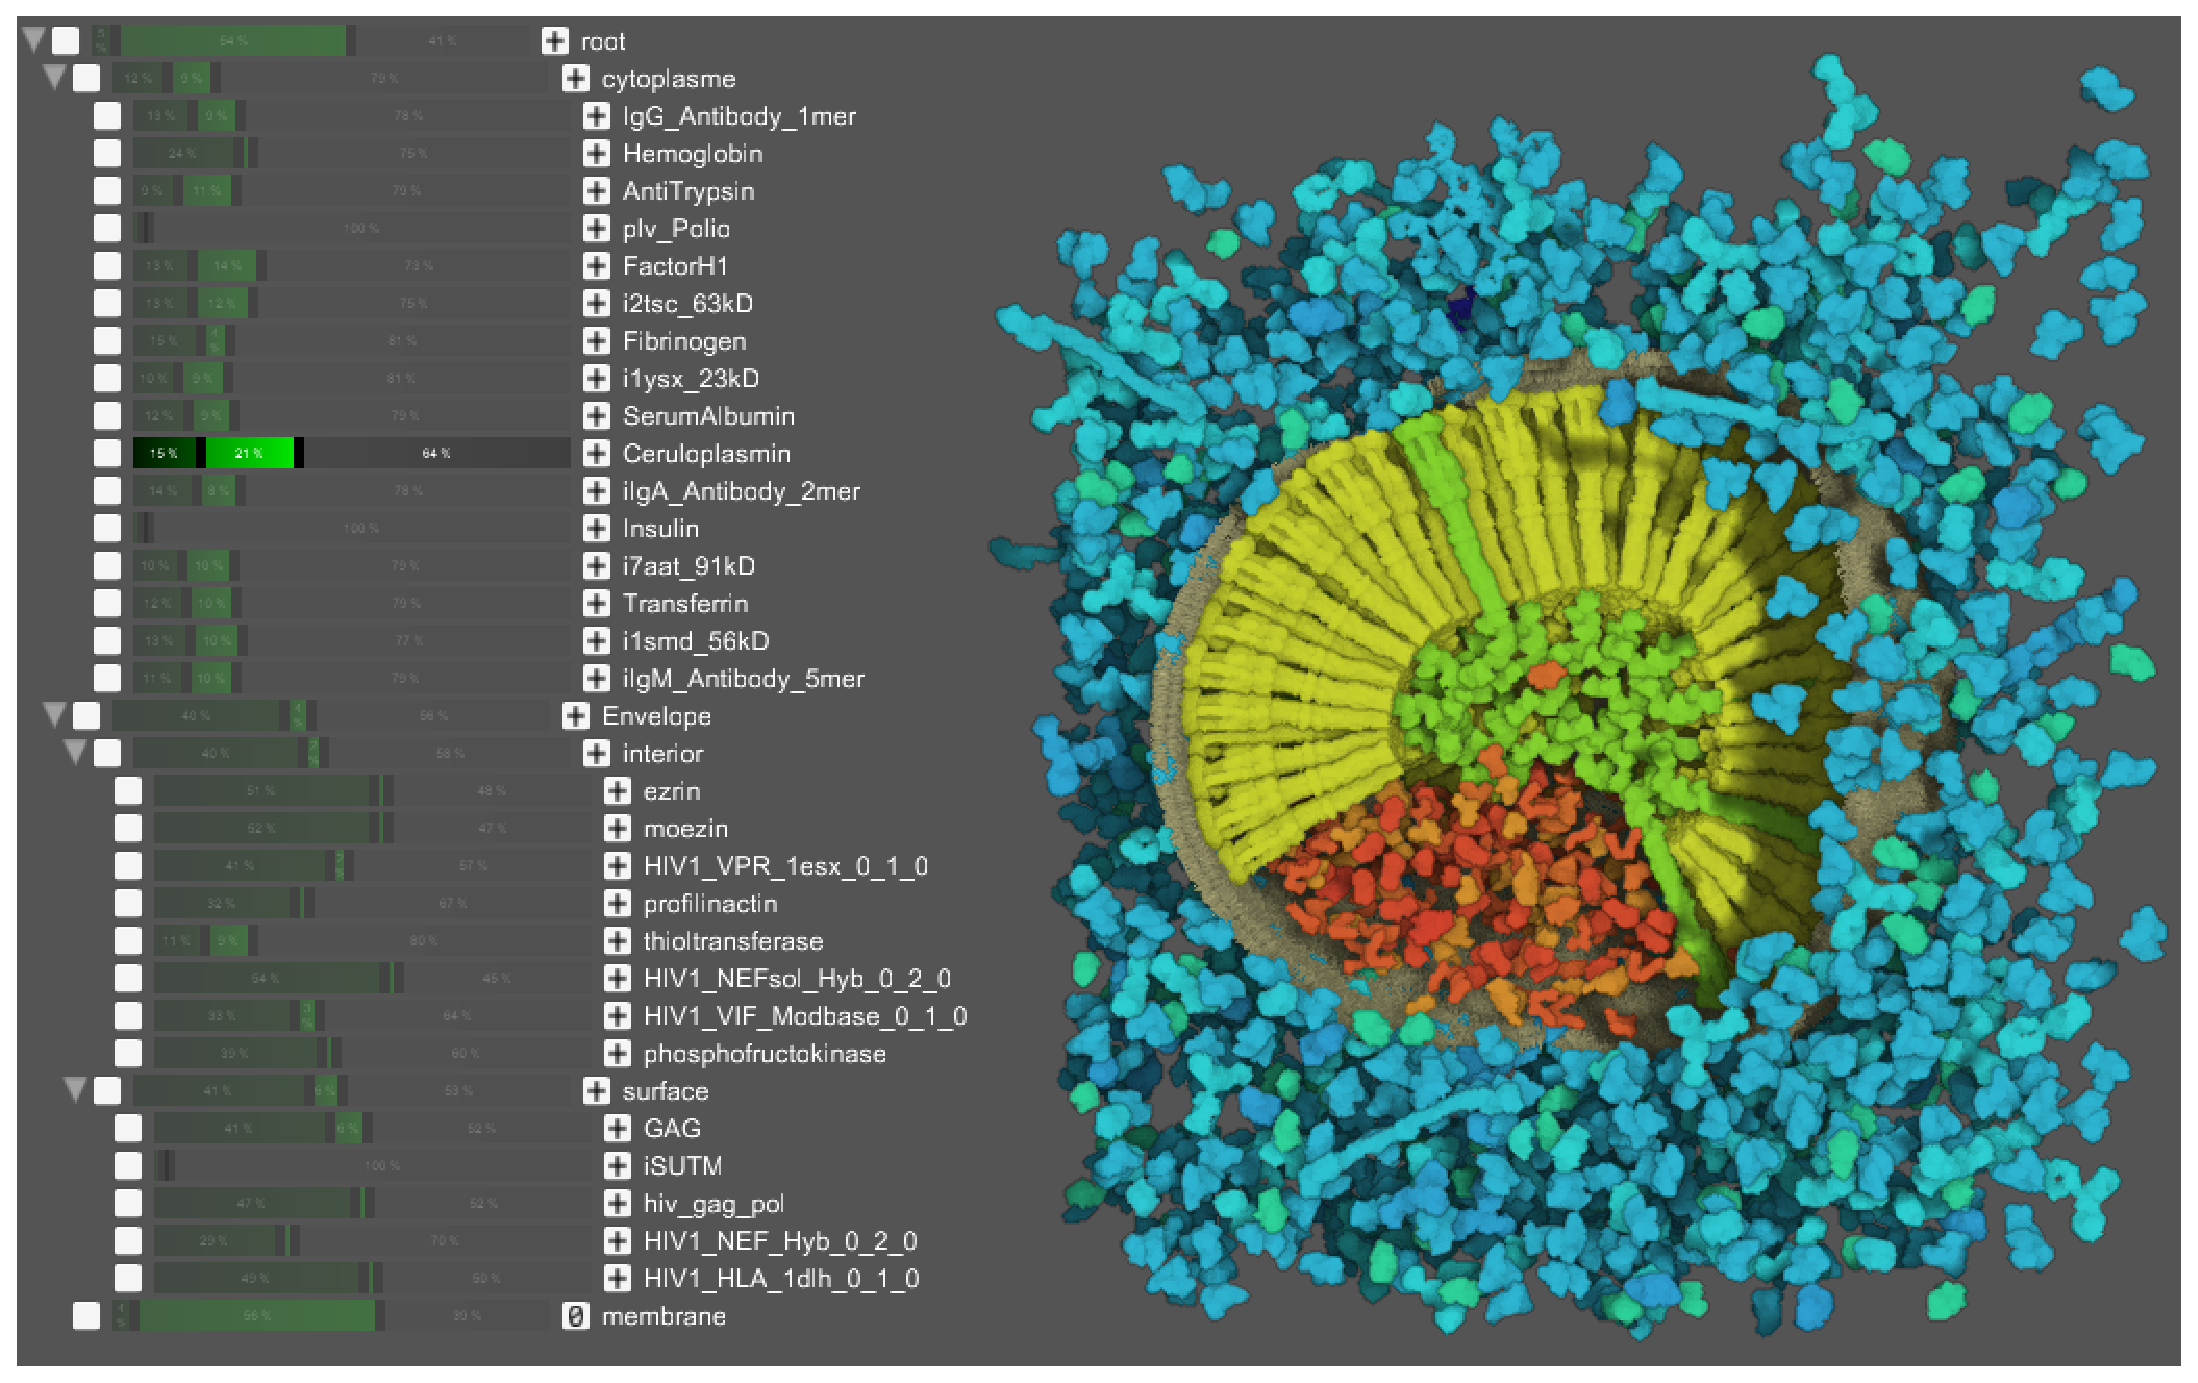
\includegraphics[width=0.4\linewidth]{figures/eq-s.eps}}
\caption{\label{fig:res:res}
Advanced clipping options in real test systems. (a) A falloff function is used to gradually clip serum molecules (red) from bottom to top to reveal the HIV capsid, with ghosting to give cues about the overall concentration. (b) Selective clipping is used to reveal the location of ribosome (blue) in a model of Mycoplasma mycoides.
(c) Internal structures of a immature HIV model are shown by several clipping objects. On the left, the visibility equalizer is shown.}
\vspace{-3mm}
\end{figure*}

The first dataset is a model of an HIV particle in blood serum that contains 20502 instances of 45 different protein types and 215559 instances of lipid molecules.
In Figure \ref{fig:res:gh3}, we show an example of a single clipping plane used to reduce the concentration of the blood serum molecules, so that the HIV proteins are visible. 
However, to avoid misleading the viewer about the actual concentration of the blood molecules, we render clipped proteins with a ghosting effect. 
This communicate true information about the concentration, while reducing visual clutter caused by the dense arrangement of blood serum proteins.
Figure \ref{fig:teaser} shows sequential step for production a comprehensible cut-away illustration with the HIV dataset.

The second dataset is a model of \emph{Mycoplasma mycoides} that contains 5380 proteins of 22 different types. 
Figure \ref{fig:res:myco} shows how fuzzy-clipping is used to reduce visual clutter to illustrate the positions of the ribosomes (shown in blue) within the cell.

The third dataset, shown in Figure \ref{fig:res:eq} is a model of an immature HIV which contains 1081 instances of 13 different protein types. 
We applied several clipping objects to reveal the internal structure of the virus. 
The blood serum (blue) has been preserved around the particle using the fuzzy clipping to illustrate how it encloses the HIV particle. 
The visibility equalizer is displayed as well, showing the ratios of visible and clipped instances of the individual molecular ingredients. 
The white boxes to the left of each stacked bar are used to mark the given ingredient or compartment as \mbox{focus}.

\begin{figure}[b]
\vspace{-4mm}
\centering
\includegraphics[width=0.89\linewidth]{figures/res-islands.eps}
\caption{\label{fig:res:islands}
HIV clipped with a plane. 
%Envelope proteins (blue) are reintroduced in the scene. 
Contextual anchoring is used to indicate the proximity of envelope proteins (dark blue) with the lipid membrane (grey)
The dark spots represent shadows projected into interior proteins.}
\end{figure}

Figure \ref{fig:res:islands} shows the mature HIV dataset clipped with a single plane. 
The contextual anchoring is applied to reintroduce parts of the clipped membrane (grey) around the envelope proteins (blue).

%\begin{figure}[t]
%\centering
%\subfloat[]{\label{fig:res:gh0}\includegraphics[width=0.5\linewidth]{figures/res-gh0.eps}}
%\subfloat[]{\label{fig:res:gh1}\includegraphics[width=0.5\linewidth]{figures/res-gh1.eps}}

%\subfloat[]{\label{fig:res:gh2}\includegraphics[width=0.5\linewidth]{figures/res-gh2.eps}}
%\subfloat[]{\label{fig:res:gh3}\includegraphics[width=0.5\linewidth]{figures/res-gh3.eps}}
%\caption{\label{fig:res:gh}The cutaway molecules are indicated through the ghosting effect. (a) Part of the scene is removed by a clipping plane. (b) The amount of cutaway molecules has been decreased through the fuzzy clipping, which caused some of the cutaway molecules to be reintroduced into the scene. (c) The blood serum (red molecules) are removed by fuzzy clipping in the entire dataset. (d) A falloff function is used to gradually change the influence of the fuzzy clipping.}
%\end{figure}
 
%Figure \ref{fig:res:gh} illustrates that this can be done in different ways according to the vision of the artist.

The visibility equalizer is designed to limit the computational overhead in order to offer a fast and responsive user experience.
To demonstrate the responsiveness of our method, we measured the computation time for the object-space clipping, view-space clipping and 2D distance transform, respectively.
The application was running on a machine equipped with an Intel Core i7-3930 CPU 3.20 GHz machine coupled with a GeForce GTX Titan X graphics card with 12GB of video RAM. 
The computation of the object-space clipping, compared to the rendering task performed by cellVIEW, is very lightweight and does not impact the overall performance too much. 
It took \textbf{0.3 milliseconds} to evaluate the 236061 instances of the HIV + blood dataset without clipping any of them.
It took \textbf{0.5 milliseconds} in total to slice the dataset in half and \textbf{0.6 milliseconds} to clip it entirely.
The increasing cost corresponds to the writing operations to the video memory, which are performed when an instance is clipped.
It is important to mention that neither the shape of the clipping object nor the number of clipping objects have a meaningful influence on the performance.

The view-space clipping, however, requires more computational work that could impact the responsiveness. 
%Therefore, a good strategy is to limit the number of view-space clipping objects, especially for very large scenes with up to several million instances. 
Indeed, for computing occlusion queries, occluders and occludees must be additionally rendered, which adds extra work to the rendering pipeline. 
For this reason, only the bounding spheres of the molecules are rendered instead of their entire structures, which may consist of hundreds or thousands of spheres, in order to guarantee a minimal computational overhead. 
We measured \textbf{0.07 milliseconds} for rendering the depth-stencil mask with 12142 instances (HIV proteins), and \textbf{0.57 milliseconds} for the computation of the 223919 occlusion queries corresponding to the remaining objects of the scene (blood proteins + lipid residues).
Additionally, the 2D distance transform that is needed for the aperture effect also requires additional computation.
It took \textbf{0.15 milliseconds} for computing the distance transform of the previous depth-stencil mask at a resolution of 512 by 512 pixels.
Unlike object-space clipping, the view-space clipping computation cost will keep increasing with additional operations.
Therefore it is a good strategy to keep a low number of view-space clipping objects, especially with very large scenes.

%\begin{figure}[t]
% \centering
%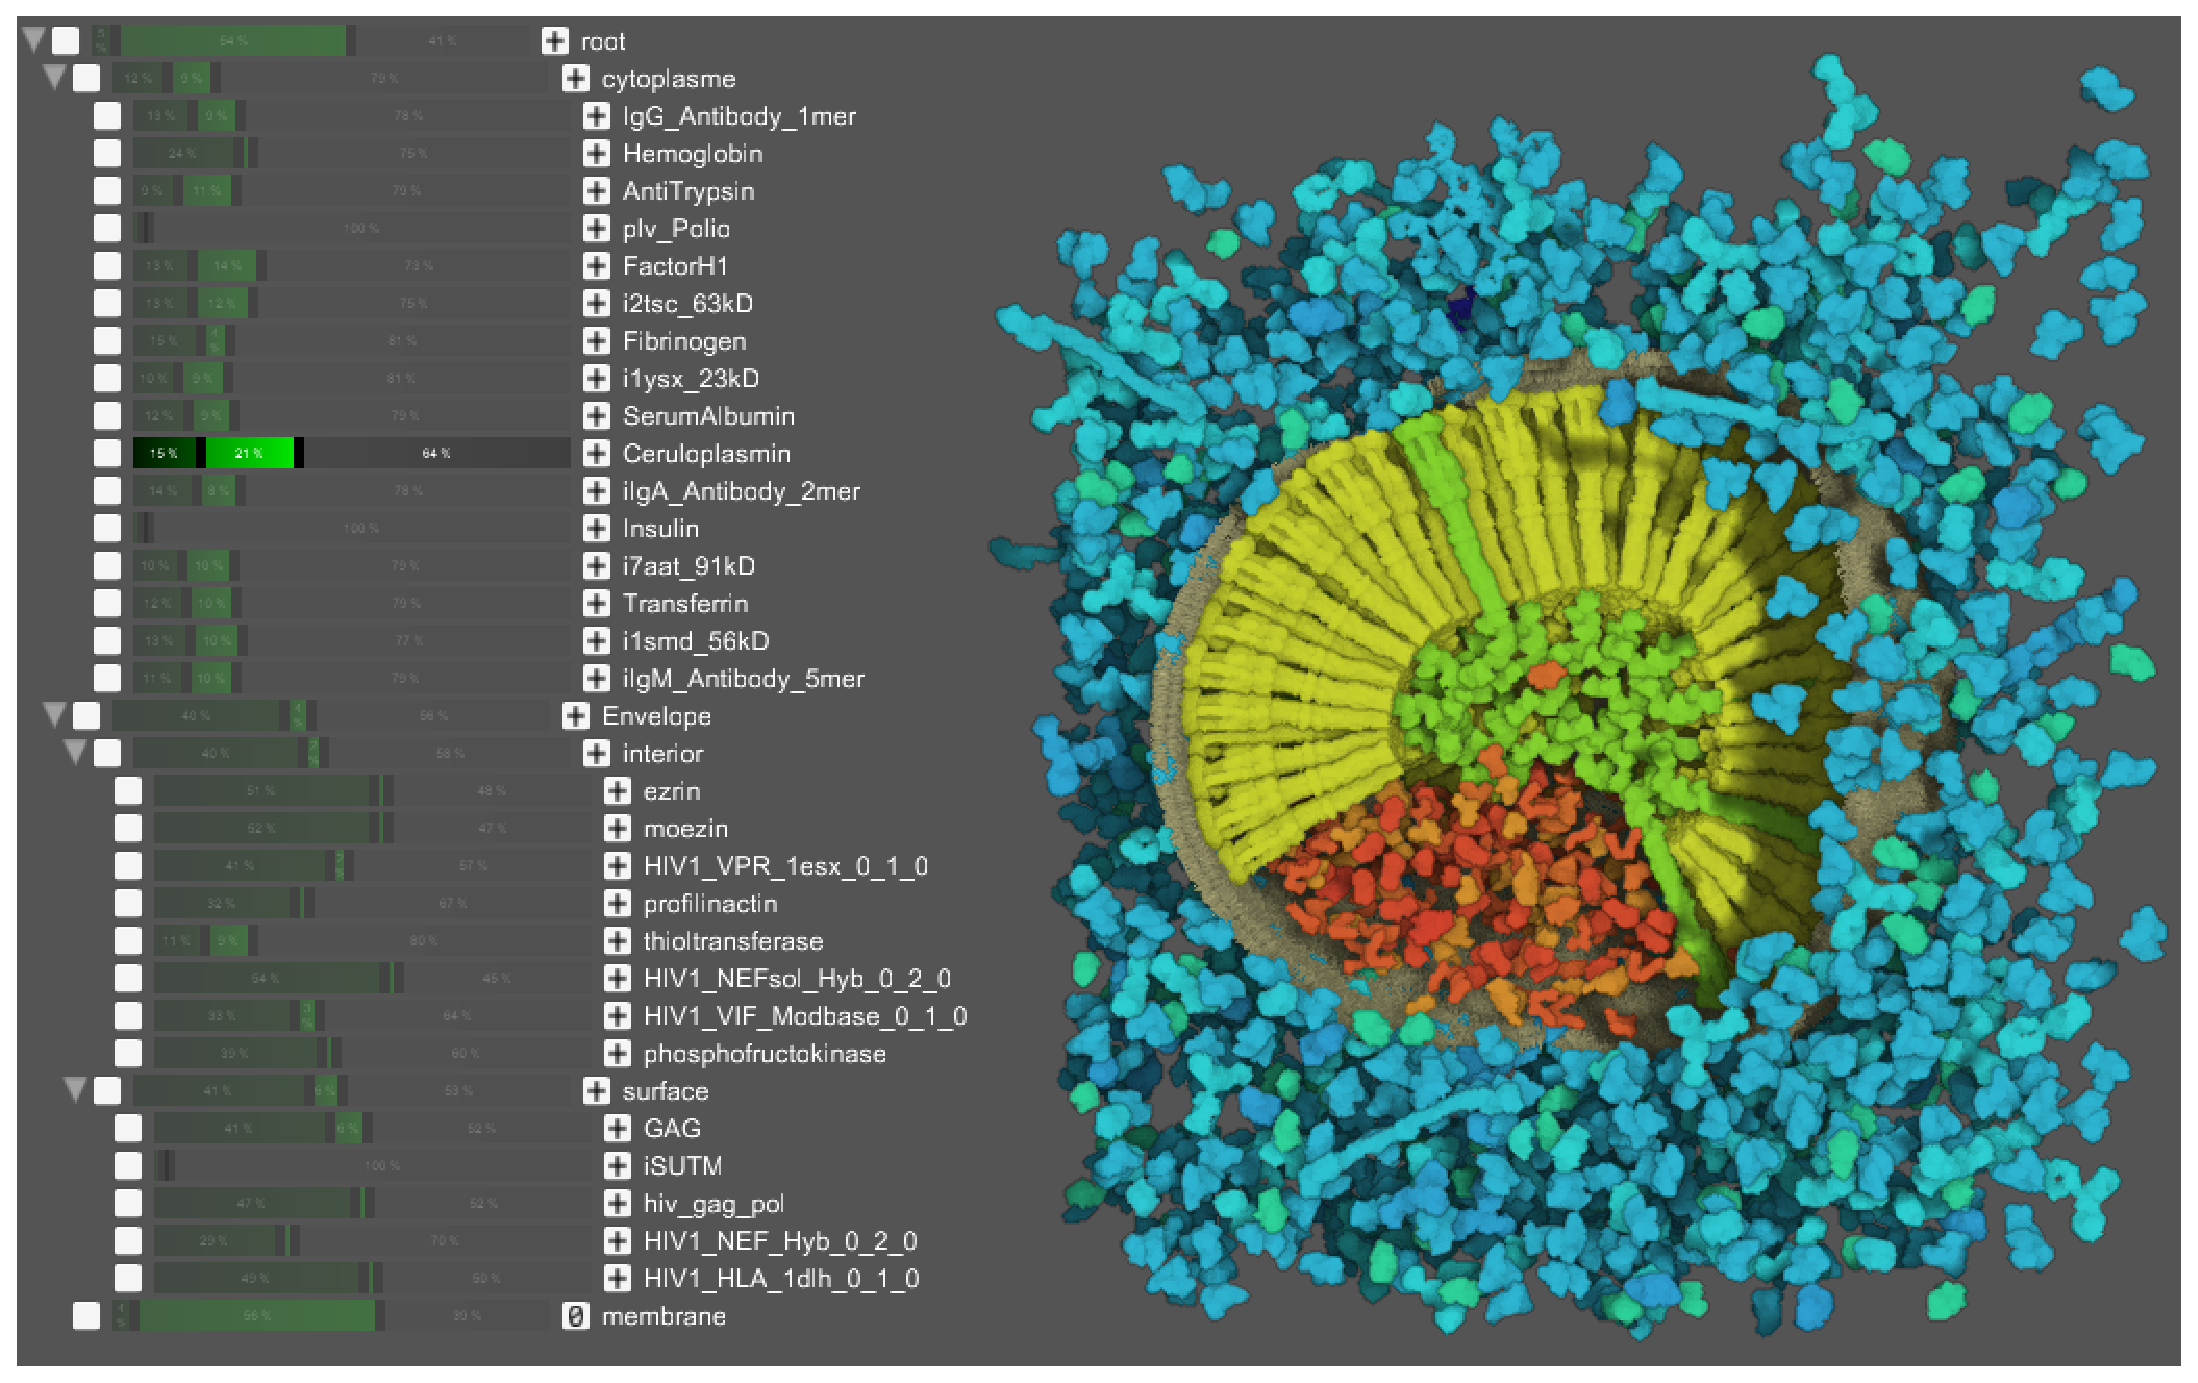
\includegraphics[width=\linewidth]{figures/eq-s.eps} %\caption{\label{fig:res:eq}Mature HIV.}
%\end{figure}


%\begin{figure}[t]
%\centering
%\subfloat[]{\label{fig:res:vsc0}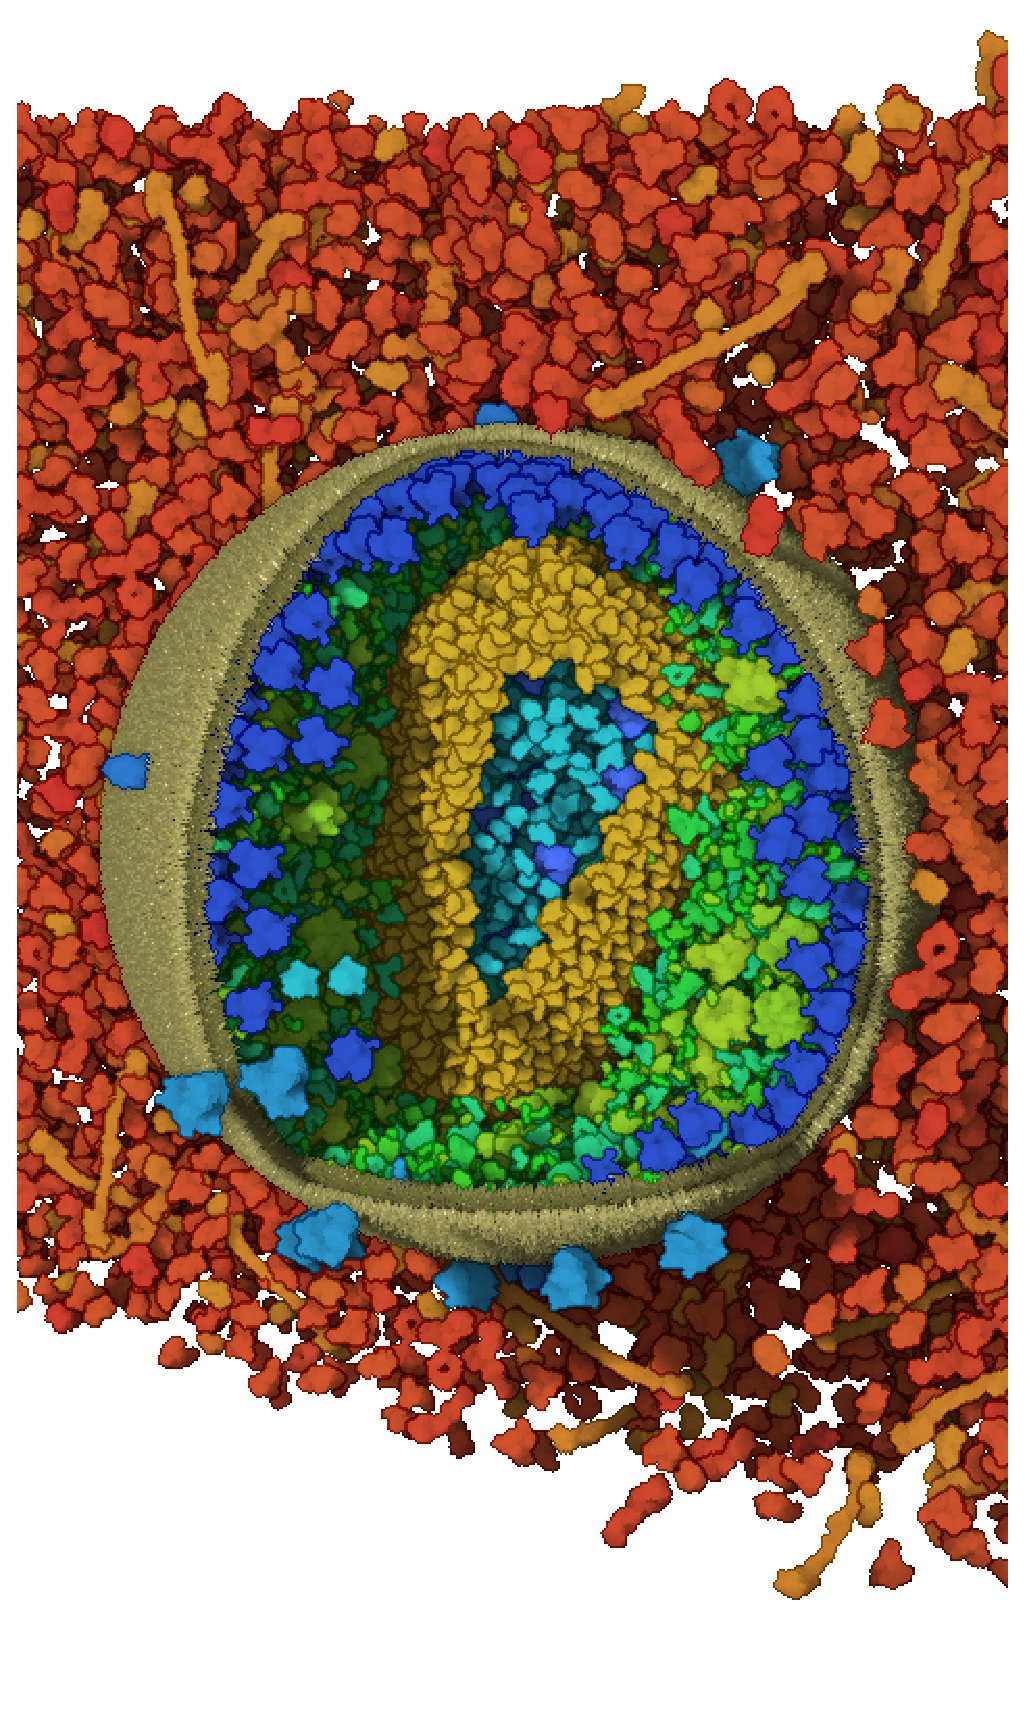
\includegraphics[width=0.245\linewidth]{figures/res-vsc0.eps}}
%\hfill
%\subfloat[]{\label{fig:res:vsc1}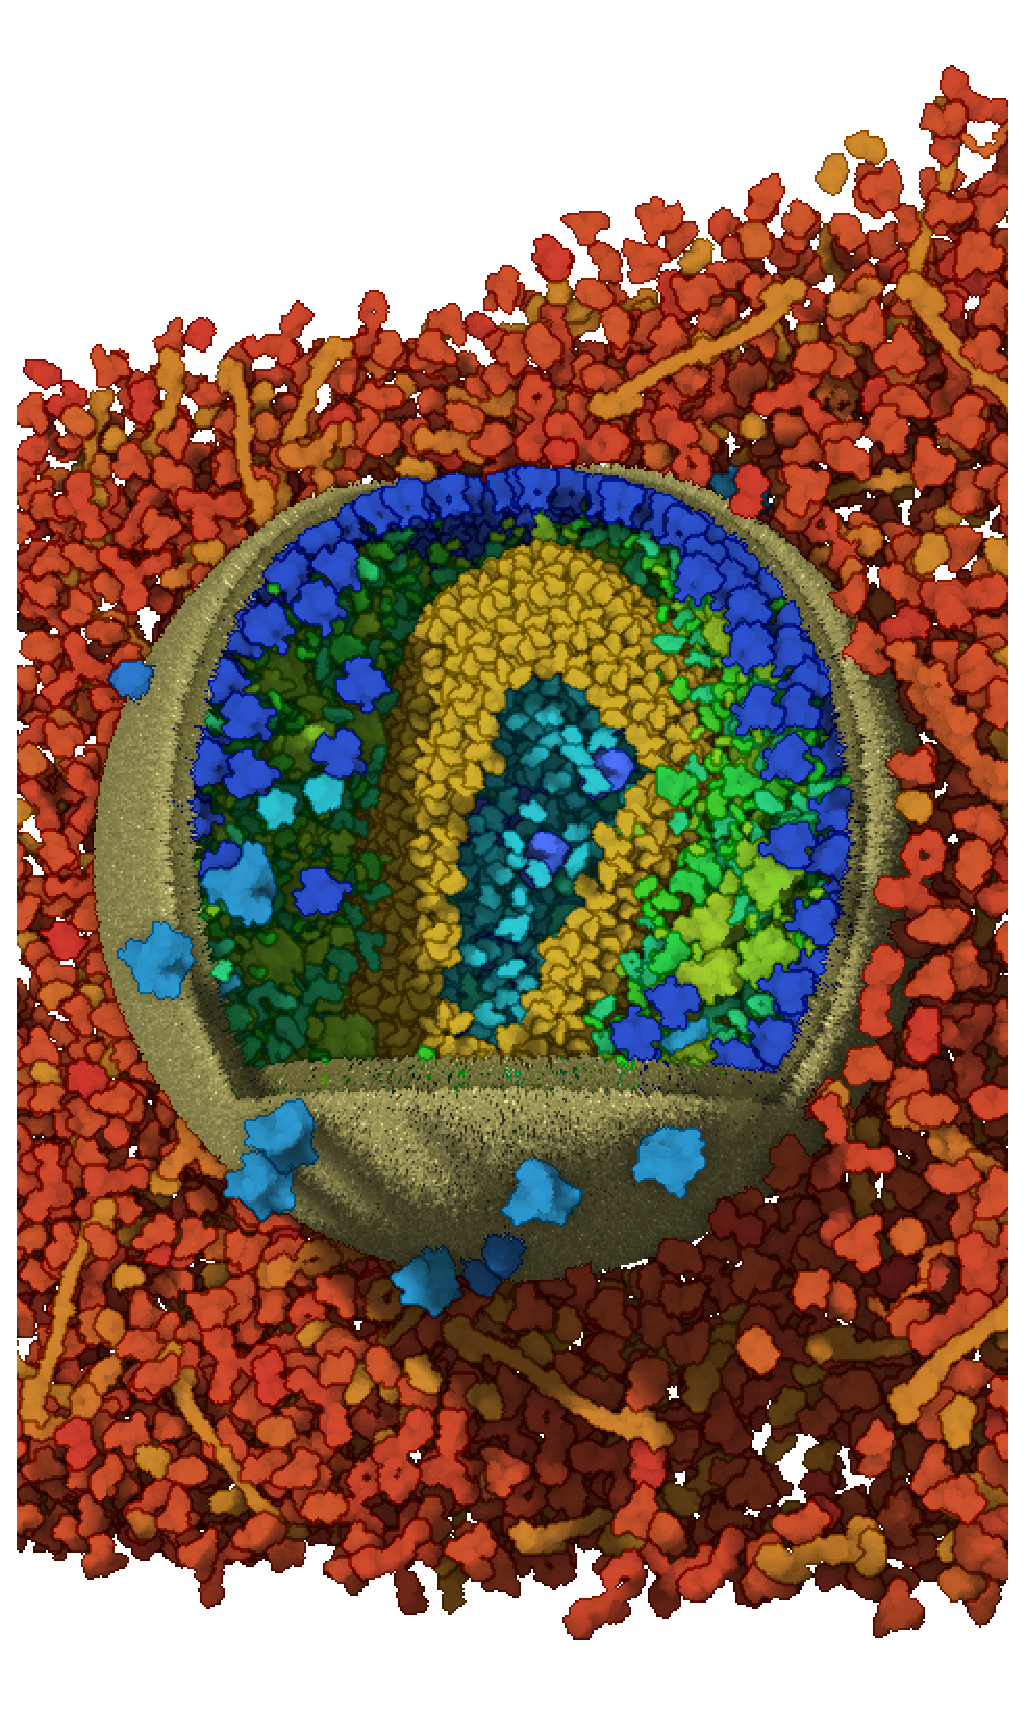
\includegraphics[width=0.245\linewidth]{figures/res-vsc1.eps}}
%\hfill
%\subfloat[]{\label{fig:res:vsc2}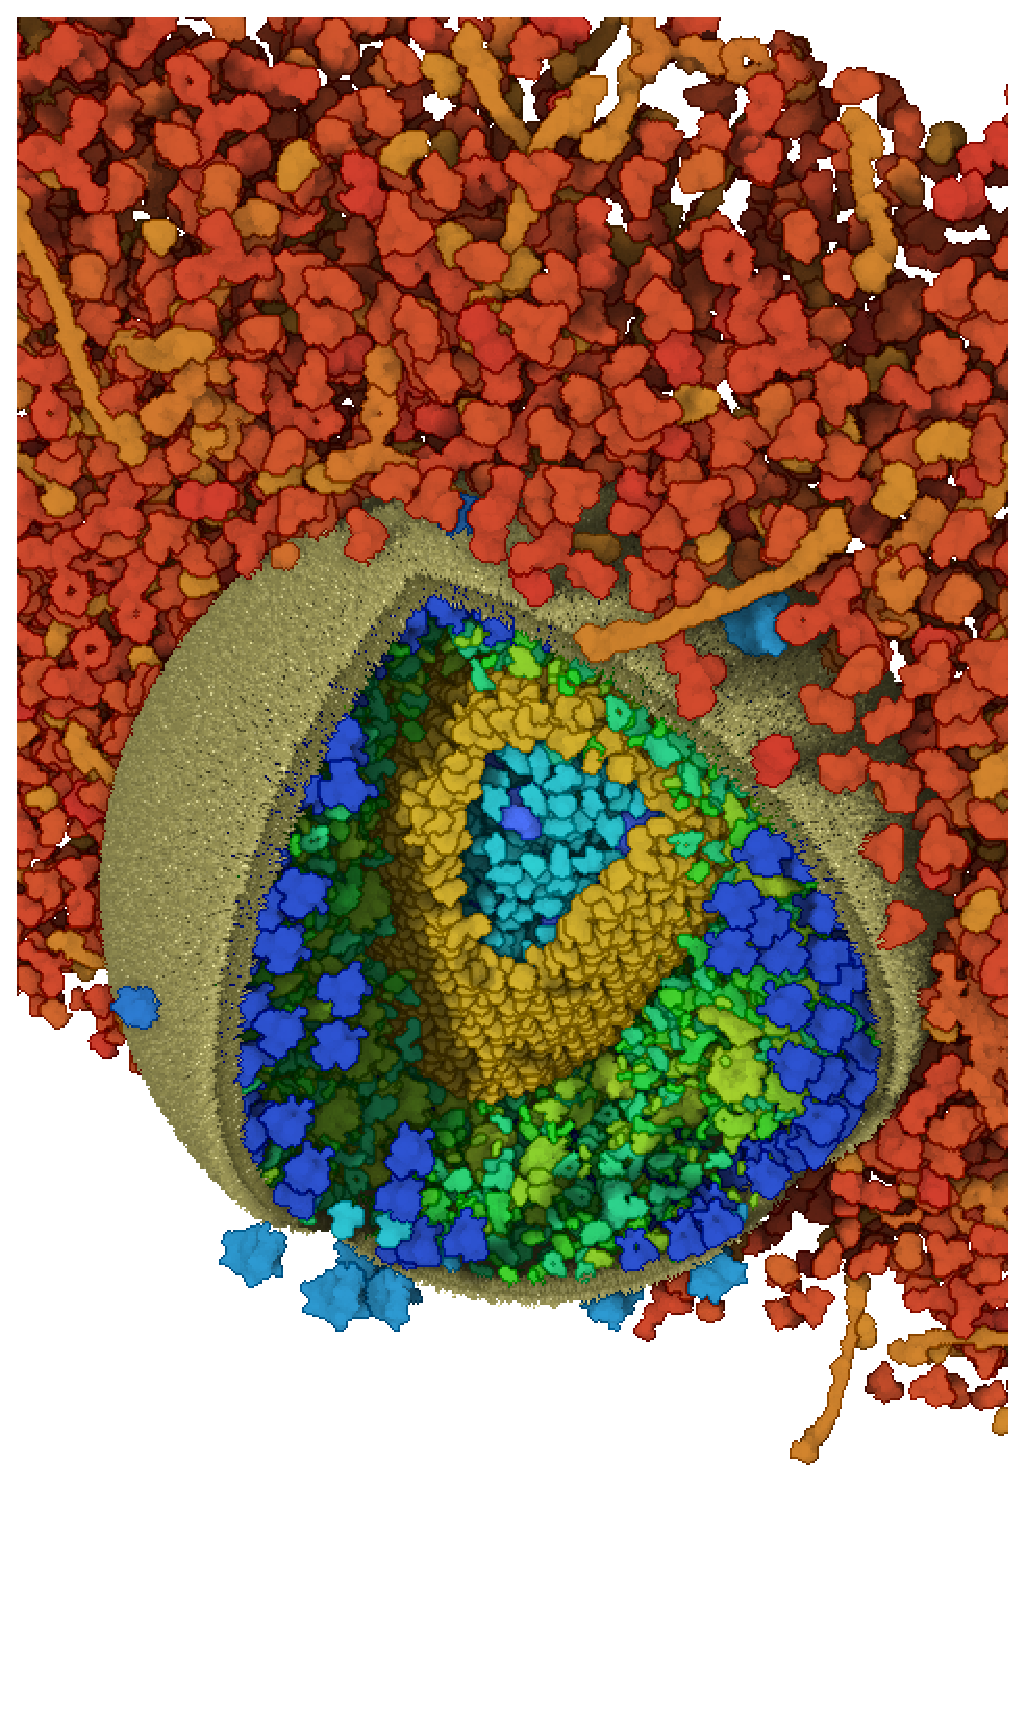
\includegraphics[width=0.245\linewidth]{figures/res-vsc2.eps}}
%\hfill
%\subfloat[]{\label{fig:res:vsc3}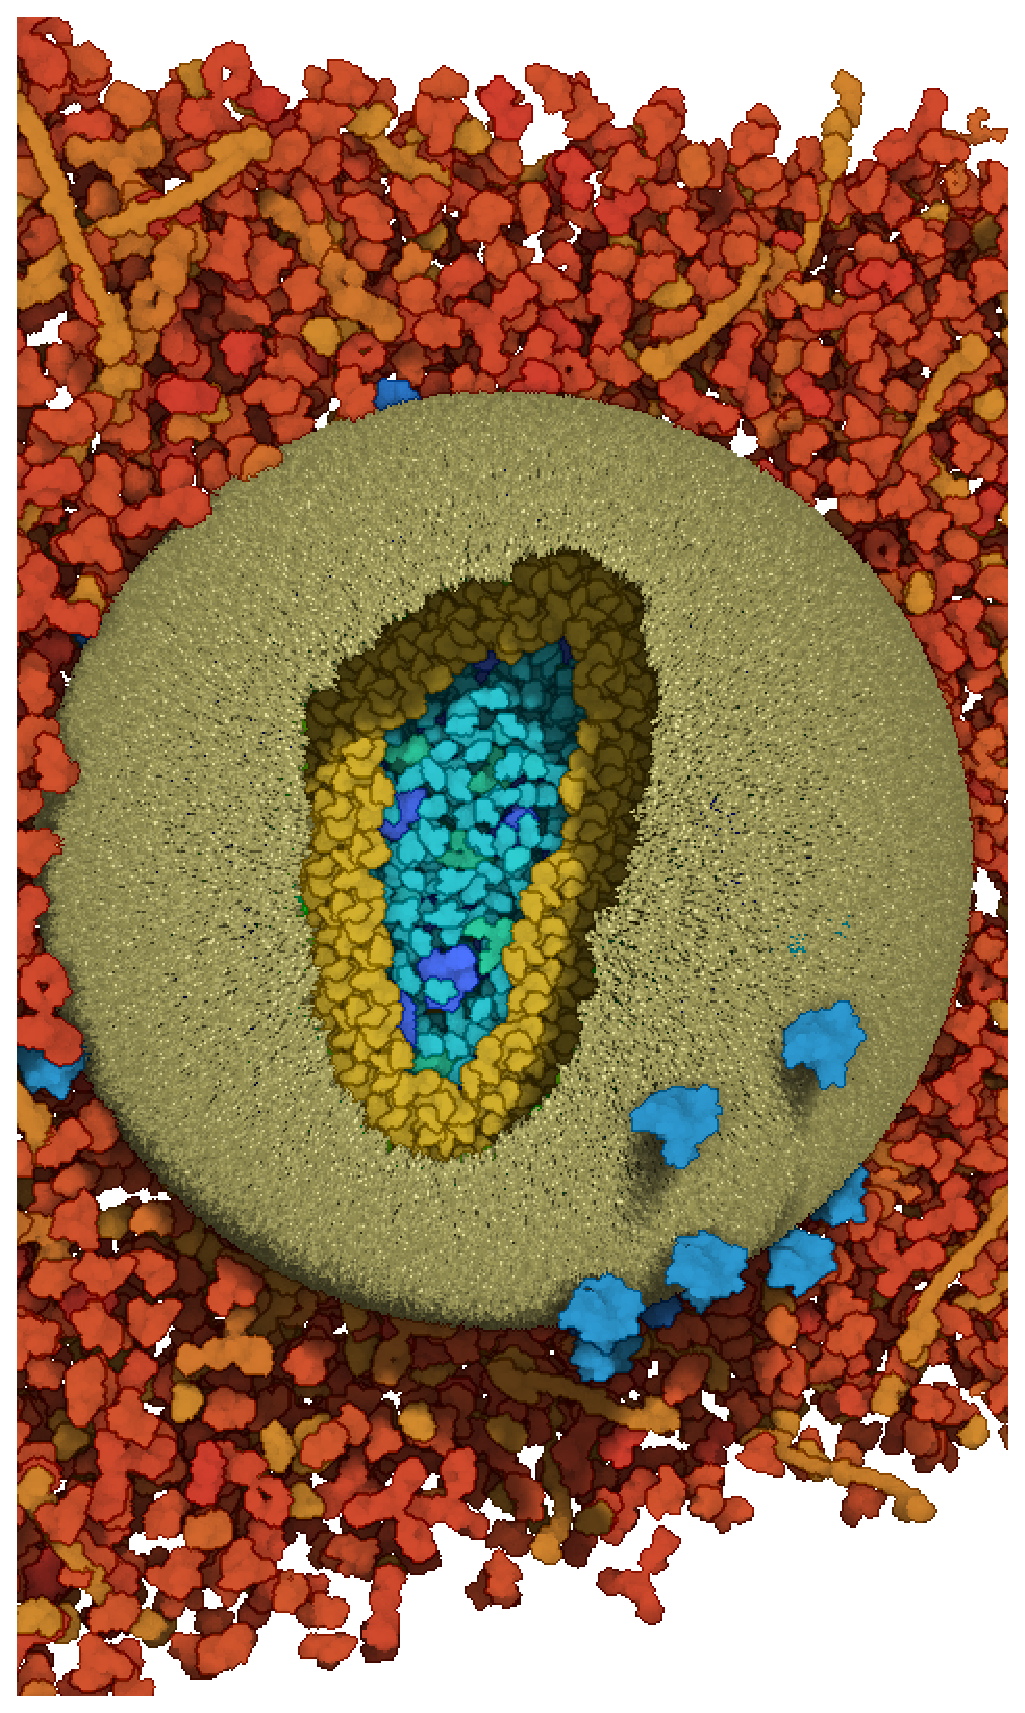
\includegraphics[width=0.245\linewidth]{figures/res-vsc3.eps}}
%\caption{\label{fig:res:gh}View-space clipping.}
%\end{figure}

%\begin{figure*}[t]
%\centering

%\subfloat[]{\label{fig:res:w0}\includegraphics[width=0.25\linewidth]{figures/res-w0.eps}}
%\subfloat[]{\label{fig:res:w1}\includegraphics[width=0.25\linewidth]{figures/res-w1.eps}}
%\subfloat[]{\label{fig:res:w2}\includegraphics[width=0.25\linewidth]{figures/res-w2.eps}}
%\subfloat[]{\label{fig:res:w3}\includegraphics[width=0.25\linewidth]{figures/res-w3.eps}}

%\subfloat[]{\label{fig:res:w4}\includegraphics[width=0.25\linewidth]{figures/res-w4.eps}}
%\subfloat[]{\label{fig:res:w5}\includegraphics[width=0.25\linewidth]{figures/res-w5.eps}}
%\subfloat[]{\label{fig:res:w6}\includegraphics[width=0.25\linewidth]{figures/res-w6.eps}}
%\subfloat[]{\label{fig:res:w7}\includegraphics[width=0.25\linewidth]{figures/res-w7.eps}}
%\caption{\label{fig:res:w}W.}
%\end{figure*}

%\begin{figure}[t]
% \centering
% \includegraphics[width=\linewidth]{figures/results01.eps}
% \caption{\label{fig:results01}An illustration of the HIV virus in the %blood serum utilizing cutaways created with our approach.}
%\end{figure}


\section{Implementation}

We implemented the pipeline within the CellVIEW framework \cite{muzic15}.


%\subsection{PoC Pipeline}
%[contains specifics about our pipeline implementation]\textbf{ [move to implementation section]}
%implemented in cellVIEW: give some details about cellVIEW): unity, supports loading \&rendering of cellPACK data, renders molecules as point clouds
%\newline

%desc was jeder component beisteuert um die beiden reps zu erzielen

\input{discussion.inc}

\input{conclusion.inc}

%% if specified like this the section will be committed in review mode
\acknowledgments{
The authors wish to thank A, B, C. This work was supported in part by
a grant from XYZ.}

\bibliographystyle{abbrv}
%%use following if all content of bibtex file should be shown
%\nocite{*}
\bibliography{trani}
\end{document}
